\documentclass{article}
\usepackage{verbatim}
\usepackage{amssymb}
\usepackage{fullpage}
\usepackage{float}
\usepackage{algorithmicx}
\usepackage{graphicx}

\usepackage[english]{babel}
\usepackage[utf8]{inputenc}
\usepackage{algorithm}
\usepackage[noend]{algpseudocode}

\newcommand\eqdist{\mathrel{\stackrel{\makebox[0pt]{\mbox{\normalfont\tiny d}}}{=}}}



\graphicspath{{figs/}}

\author{
  Roberts, Lucas\\
  \texttt{rlucas7@vt.edu}
  \and
Giese, W. Gill \\
  \texttt{giese@vt.edu}
}

\date{\today}
\setcounter{table}{0}

\begin{document}
\title{
Why Nematologists Should Use Zero-Inflated Models with Count Data And How To Use Them
}

\maketitle

\begin{abstract}
Zero-inflated models are an essential yet seldom used tool by nematologists when modeling abundance data. Traditional sample means are inadequate estimators when excessive zeroes exist in the measurement counts. We show that using sample means when zero-inflation is present leads to a bias in the rate estimate causing scientists to underestimate the rate of nematodes in a soil sample. Moreover, we show that even if the nematologist collects a very large number of measurements, the error will persist. A test is provided which aids the scientist in determining the presence of zero-inflation. Additionally, an algorithm is given for estimation of the zero-inflation probability via a programmable spreadsheet. We provide a table of common statistical software with relevant information for the scientist to focus their software choice and how to use the chosen software. 
\end{abstract}

\section{Introduction}
Raw nematodes counts, abundance measures, and rates within a unit volume of soil are all common measures of nematodes. The method of counting after elutriation is time consuming but conceptually straightforward for the researcher. In our own work \cite{giese2016cover} we found count models of root measures in vineyards to be inadequate statistical models for these observed data. The count data are often observed with a high prevalence of zeroes, indeed often beyond the frequency of zeroes suggested by the Poisson model itself. In cases with excess zeroes the Poisson model is inadequate to estimate the true, underlying rate of nematode abundance. Zero-inflated models offer an alternative that accounts for the excess zeroes observed as well as providing additional over dispersion flexibility. A distribution is called over-dispersed (relative to the Poisson) if the variance exceeds the mean, $\sigma^2 > \mu$. 

In many cases nematologists, and scientists in general use the Poisson model not because it is appropriate for the observed data but because the scientist is familiar with the modeling approach of calculating sample means. When analyzing count data to obtain an estimate of the rate per unit, using a sample mean to estimate the rate is equivalent to assuming a Poisson count distribution. This article is meant to bring the zero-inflated models to the attention of scientists who model nematode abundance data and point out the pitfalls of using traditional methods in the presence of excess zero counts. The use of zero inflated models is common in other disciplines such as dentistry \cite{bohning1999zero}, road accidents \cite{shankar1997modeling}, and software faults \cite{khoshgoftaar2001application}. The zero-inflated Poisson model has been seen in the analysis of nematode count data by Murray et al. \cite{murray2011modeling}. Murray et al. mentioned that the zero-inflation might come not from the lack of nematodes but from the symbiotic relation between certain species (southern root knot) and the root system, once the nematode embeds in the root system there is limited ability to measure the organism. The only time the organism may be measured is when recently-hatched larvae are detectable in the soil prior to invasion \cite{murray2011modeling}.

There are many readily available software applications for fitting zero-inflated models. We provide a table of common statistical software to fit zero-inflated models and compare relevant aspects of these software applications. Moreover, for the scientist who prefers to `cook their own' statistics we also provide a spreadsheet on the publisher's website so that the scientist may perform the calculations on simplified zero-inflated Poisson models themselves. Also the spreadsheet serves as an instructional aid. The scientist may study the formulae and calculations to ensure their understanding of the model and resulting calculations.  

Beyond the statistical aspects of zero-inflated models for count data, there are very important scientific considerations for using these models. One salient consideration is that failing to use zero-inflated models when the data are in fact zero-inflated leads to a bias in the estimated rates of nematodes per unit volume of soil. The reported rate estimates determined under the traditional (sample average) models will underestimate the rate parameter and may cause a grower to fail to act when in fact they should make efforts to control their nematode population either by rootstock selection, sanitation of field implements, and other mitigation methods like methyl bromide fumigation and beyond, as outlined by Zasada et al. \cite{zasada2010managing}.  Additionally, the scientist might assume that as long as they collect a sufficient number of samples the bias from misspecifying the Poisson model will be negligible. We show that the bias persists for any large number of measurements and a larger rate implies a larger error in estimation. 

The remainder of this manuscript proceeds as follows. Section \ref{sec:est} discusses the theoretical challenges of rate estimation and presents the bias results for zero-inflated data. Section \ref{sec:model_det} gives a test statistic for the researcher to determine whether to use a zero-inflated or a Poisson model. Section \ref{sec:algo} presents an EM algorithm to estimate the two parameters in a ZIP model. Also, we give a link to an excel spreadsheet where the algorithm is already programmed. Section \ref{sec:zip_soft} lists a table with comparisons of various software that may be used to fit a zero-inflated Poisson regression model. Finally, Section \ref{sec:disc} concludes with a discussion and summary of the manuscript. 

\section{Estimation challenges}\label{sec:est}

The bias of an estimator is defined as the difference between the expected value of the estimator and the parameter to be estimated. In the case of count data often the researcher wants to know the rate parameter which indicates an average number of nematodes per unit of soil volume. Let the rate parameter be denoted $\lambda$ and let the zero inflation probability be denoted $\phi$. If the researchers use the average of the counts, denoted $\bar{y}$, and the data are in fact distributed according to a ZIP distribution then the expected value of the sample mean is 

\begin{equation}\label{eqn:bias}
\mathbb{E}(\bar{y}) = (1-\phi)\lambda.
\end{equation}
Thus the bias of the estimate is 

\begin{equation}
\underbrace{\mathbb{E}(\bar{y}) - \lambda}_{=bias} = -\phi\lambda,
\end{equation}
so that the larger the zero-inflation or the rate parameter, the larger in real terms, the bias of the estimate. 

One common approach to analyzing excess zeroes in count data is to add 1 to each observed count. If the counts are indeed Poisson distributed, the resulting random variable is a size-biased Poisson \cite{arratia2013size,arratia2010size}. Regardless of the underlying distribution if you use the counts with 1 added to each, then the rate estimate will be biased by 1. To remove this bias you may safely subtract 1 from the average. Note that this does not solve the problem of excess zeroes nor does the procedure alleviate the bias of the estimator detailed above. Another common method especially when analyzing abundance data (e.g. \cite{jagdale2013incidence}) is to condition on the count being greater than zero  which is equivalent to ignoring the zero counts. Under a ZIP distribution one can show that the distribution $\Pr(Y=y \vert y>0)$ has a zero-truncated Poisson distribution. For more on the statistical properties of this distribution see Cohen \cite{cohen1960estimating} and Singh \cite{singh1978characterization}. Unfortunately, the sample mean is a biased estimate of the rate parameter $\lambda$ in this zero-truncated case as well. Moreover, some authors prefer to use a transformed version of the count with a 1 added. Some examples are $log(y+1)$ \cite{howland2014spatial,centinari2016root} or $\sqrt{2(y+1)}$ \cite{anscombe1948transformation,yu2009variance} and similar variations to these two transforms. Both of these transforms lead to biased estimators of the underlying rate. The second transform which uses a squared root, has origins in the variance stabilization literature \cite{freeman1950transformations} and would be reasonable without the addition of a 1 \emph{only if the underlying counts are Poisson distributed}. In the applied papers where these transforms were applied, no likelihood ratio test to check the Poisson assumption was applied.

Of course the researcher might reasonably assume that with enough measurements, the bias is not a problem. This assumption is known as asymptotic unbiasedness in the statistics literature. We now detail that this assumption, although reasonable, is erroneous. 

Perhaps the most common measure of the closeness of an estimator to the true parameter is the mean squared error (MSE). The MSE is defined as the expected value of the squared difference between the estimator and the true value of the parameter. Formally written, 
\begin{equation}
MSE(\bar{y}, \lambda) = \mathbb{E}(\bar{y}-\lambda)^2,
\end{equation}
We use the well-known bias variance decomposition of the MSE equation to calculate MSE in this case and we use the conditional variance formula for calculating the variance of the ZIP random variable. The bias has already been given above in Equation \ref{eqn:bias}. The MSE for the average as an estimator of the rate is 
\begin{equation}
MSE(\bar{y}, \lambda) = \phi^2\lambda^2 + \frac{ \lambda(1-\phi) +\lambda^2(1-\phi)\phi}{n}.
\end{equation}
This last equation tells us that even with an infinite number of samples ($n \to \infty$) unless the zero-inflation is non-existent, there will be a bias proportional to the square of the (true) rate and the traditional methods will be suboptimal to use in place of estimators of zero-inflation. This section has discussed the statistical estimation of rates for data which are truly zero-inflated. In practice we never know for certain whether the data are truly zero-inflated or not and we must rely on statistical tests to make this determination. The next section discusses a method to make the Poisson or ZIP determination as well as a statistical nuance of the procedure.
 
\section{Model determination: Poisson or ZIP?}\label{sec:model_det}

There are two commonly used methods to determine whether the count data you are modeling is from a zero-inflated distribution or not: the likelihood ratio (LR) test and the Vuong test \cite{vuong1989likelihood}.  
There is a fair amount of disagreement within the scholarly community about when to use the Vuong test or the LR test \cite{wilson2015misuse} in zero-inflated models. Notwithstanding these disputes, the Vuong test is actually a class of tests that are appropriate when comparing two zero-inflated regression models that may or may not be nested. We will not detail the Vuong test for reasons of scope but the interested reader is referred to the original paper by Vuong as well as two econometrics textbooks \cite{2005estimation,davidson1995estimation}. The likelihood ratio test method is appropriate when comparing a Poisson model against a zero-inflated model. We will not detail the likelihood ratio test but rather give an asymptotically equivalent test known as the score test. We detail the score test because the form of the test statistic is simple, intuitive and easily calculated. The formula for the score statistic is

\begin{equation}
S_n = \frac{(n_0 - np_0)^2}{np_0(1-p_0) - n\bar{y}p_0^2},
\end{equation}
where $n_0$ denotes the number of observations recorded 0, $n$ is the total number of observations including the zeroes, $p_0$ is an estimate for the probability of observing a zero in a Poisson distribution, and $\bar{y}$ is the sample mean of all counts including the observed zeroes \cite{van1995score}. A common estimate for $p_0$ would be to use $\exp(-\bar{y})$, although the alternative estimator $(1-1/n)^{n\bar{y}}$ is also reasonable. Both estimates give very similar answers in most cases. If the observed counts are truly Poisson distributed then the test statistic $S_n$ will be distributed according to a chi-squared distribution with 1 degree of freedom. We provide a table with common critical values for the chi-squared with 1 degree of freedom in Table \ref{tab:table1}. 

The score test statistic is constructed by taking the derivative of the log-likelihood with respect to the parameter(s) assuming the null hypothesis is true. In our case the likelihood is a ZIP distribution. We parametrize in terms of the odds $\theta = \phi /(1-\phi)$. Then the score function for $\theta$ is

\begin{equation}
\sum_{i=1}^n \left( \frac{-1}{1+\theta}+ \mathbb{I}(y_i=0)\frac{1}{(\theta+\exp[-\lambda_i])}\right).
\end{equation}
One can readily check that the expected value of the score equation above is 0 when summed over all observations by using $\mathbb{E}(\mathbb{I}(y_i=0))=(\theta+e^{-\lambda_i})/(1+\theta)$. Note here the notation $\mathbb{I}(A)$ is an indicator function which takes the value 1 when the event $A$ occurs and 0 otherwise. Using standard results in statistics, this score statistic will be asymptotically distributed with a chi-squared distribution with 1 degree of freedom. The score test \emph{will} converge to the chi-squared distribution because the zero-inflation parameter ($\phi$) does not have a boundary at the value 0 as is commonly assumed but at the value $-e^\lambda/(1-e^\lambda)$. For cases when $\phi$ is less than 0 the term zero-inflated may not accurately describe reality because we are reducing the probability of the 0 values to a smaller probability than would be assumed with a Poisson distribution. The case when the likelihood ratio statistic has a parameter on the boundary of the parameter space is a well studied and understood problem within statistics that occurs in other models as well, such as a mixed effect model when you want to test whether one of the variance components is 0 or not \cite{crainiceanu2004likelihood}. In boundary cases the results state that the distribution of the test statistic has probability one-half at the zero point and then other one-half probability is spread over a chi-squared distribution with a single degree of freedom \cite{chernoff1954distribution,feng1992statistical,self1987asymptotic}. Table \ref{tab:table1} gives the critical values of the chi-squared distribution for common type 1 error rates. 

\begin{figure}[H]
\label{fig:twice_log_likelihood}
\vspace{0.5in}
\begin{center}
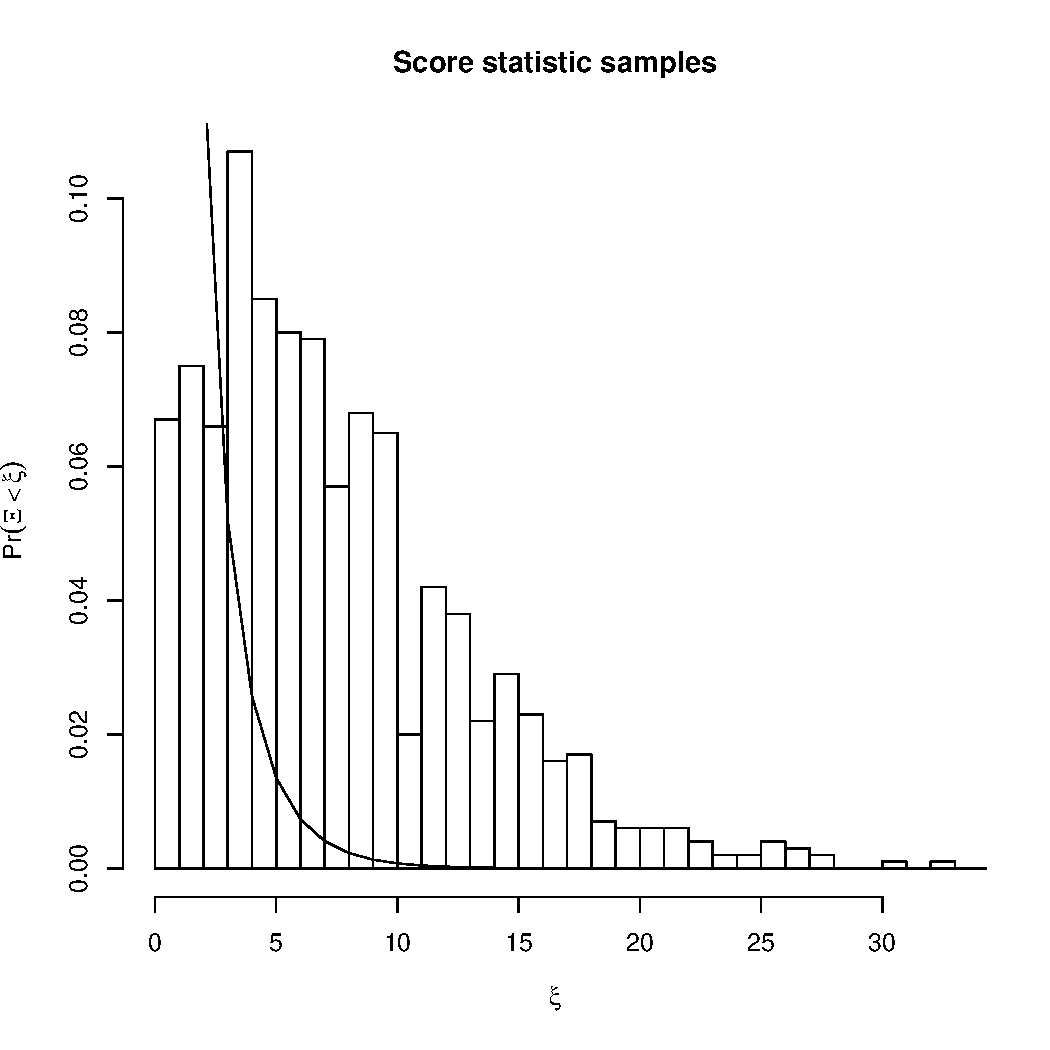
\includegraphics[scale=0.6]{hist.pdf}
\caption{Simulated and theoretical values of the score statistic with Poisson random variables.}
\end{center}
\end{figure}

\begin{table}
\begin{center}
\begin{tabular}{llr}
\hline
\multicolumn{2}{c}{Score test values} \\
\cline{1-2}
P-value & Critical value $\xi$ \\
\hline
0.001 & 0.682447\\
0.01 & 0.680257\\
0.025 &0.676564\\
0.05 &0.670281\\
0.1 &0.657218\\
0.25 &0.613524\\
\hline
\end{tabular}
\end{center}
\caption{The critical values of the score test. }
\label{tab:table1}
\end{table}

\section{An algorithm for estimating $\phi$ and $\lambda$ with no covariates}\label{sec:algo}

In this section we detail an algorithm for estimating the two parameters of a ZIP model that is readily programmable within a spreadsheet with basic arithmetic calculations. Although the algorithm contains a while loop that is potentially infinite, in our experience the number of iterations until the algorithm converges is typically no more than 20. Moreover, the calculations required in each iteration are readily programmed so that the researcher may apply the technique to various data via copy and paste to mimic the iterations of the while loop. The algorithm follows: 

\begin{algorithm}
\caption{ZIP EM algorithm}\label{alg:zip_em}
\begin{algorithmic}[1]
\Procedure{ZIP EM}{$\phi^0,\lambda^0, \varepsilon, \vec{y}, \vec{w}$}
\For{$i \gets 1, n$}
 	\If{$y_i =0$}
  		\State $w_i \gets (1+\exp[-\lambda_i^0 -\textnormal{log}(\phi_i^0/(1-\phi_i^0))])^{-1}$ 
	\Else 
  		\State $w_i \gets 0$ 
 	\EndIf
\EndFor
\State $t \gets 1$
\While{$\varepsilon > \vert\phi^t - \phi ^{t-1}\vert$ and $\varepsilon > \vert\lambda^t - \lambda^{t-1}\vert$}
\State $\phi^t \gets \sum_{i=1}^nw_i/n $\\
\State $\lambda^t \gets \sum_{i=1}^n(1-w_i)y_i /\left(\sum_{i=1}^n(1-w_i)\right) $\\
\For{$i \gets 1, n$}
 	\If{$y_i =0$}
  		\State $w_i \gets (1+\exp[-\lambda_i^t -\textnormal{log}(\phi_i^t/(1-\phi_i^t))])^{-1}$ 
	\Else 
  		\State $w_i \gets 0$ 
 	\EndIf
\EndFor

\State $t\gets t+1$\\
\EndWhile
\State \textbf{return} $\phi^t, \lambda^t$\Comment{The EM algorithm (MLE) estimates}\\
\EndProcedure
\end{algorithmic}
\end{algorithm}
The algorithmic description is a formal way of stating the procedure to get the estimates which in essence involves iterating the calculations on lines 9 and 11 and updating the weights ($w_i$) in lines 15 and 17 after a first initialization of the relevant values. For initial values of $\phi^0, \lambda^0$, and $\vec{z}$, we suggest random uniform numbers between 0 and 1 for all three. Note that final values output by the algorithm for $w_i$ and $\phi^t$ will be between 0 and 1 while $\lambda^t$ may be any positive value. Although a while loop with a stopping condition on the successive estimates of the rate and zero-inflation parameters is formally used in the algorithm, often replacing the stopping conditions with $t<10$ or another sufficiently large whole number of iterations is sufficient for many reasonable settings of numerical accuracy ($\varepsilon$). 

A spreadsheet to accompany the manuscript is available to illustrate the necessary calculations as well as provide a working template for the nematologist. The spreadsheet is titled \texttt{zip\_calcs.xlsx} and is available in the supplementary material. In the spreadsheet we use a two significant digit stopping rule and we also calculate the score statistic. The data provided in the spreadsheet are simulated Poisson variates so the score statistic has a large pvalue indicating evidence in favor of the null hypothesis that the data are distributed Poisson. Nonetheless, for illustrative purposes we proceed with the zero-inflated Poisson algorithm calculations so that the reader may study the calculation procedure. Also this example provides evidence that the algorithm provides a reasonable answer in the case of Poisson data, a small ($\phi \approx 0.03$) zero inflation estimate. 

\subsection{Numerical Example} 

In this section we present the calculation of the score statistic to determine zero-inflation status and then use the test outcome to determine the method of estimating the rate and-if applicable-the zero-inflation probability. 

First consider the summary data in Table \ref{tab:table_zip_data} although some of the calculated statistics are redundant we include them in the table for completeness. The sample mean row may be calculated using the formula $\sum_{i=1}^ny_i/n$. 

\begin{table}

\begin{center}
\begin{tabular}{c | c l c  c  c  c  }
\hline
\multicolumn{6}{c}{Species} \\
\cline{1-6}
& stunt & spiral & ring  & dagger & rootknot \\
\hline
$n$& 144 &144  &144 &144 &144  \\
$n_0$ &54  & 12 &135 &59 & 121 \\
$\sum_{i=1}^ny_i$ &12360 & 38120 & 420&4620 &1920 \\
$\bar{y}$ &85.93 &264.72  &2.92 & 32.08& 12.33 \\
$S$ &$3.83\times10^{38}$ &$9.28\times10^{114}$ & $2.64\times10^3$ &$2.07\times10^7$ &$6.28\times10^7$  \\
\hline
\end{tabular}
\end{center}
\caption{Summary statistics for example zero-inflated Poisson analysis. }
 \label{tab:table_zip_data}
\end{table}

First let us consider the stunt species. Recalling the formula for the score test statistic,

\begin{eqnarray}
S_n &= \frac{(n_0 - np_0)^2}{np_0(1-p_0) - n\bar{y}p_0^2}\\
&= \frac{(54 - 144\times e^{-85.94})^2 }{144\times e^{-85.94}\times (1-e^{-85.94}) - 12360\times e^{-2\times85.94} }\\
&= \frac{2.92\times10^{3}}{7.61\times10^{-36}}\\
&\approx3.83\times10^{38}
\end{eqnarray}

Depending on how many significant digits are kept in the intermediate steps of the calculation the test statistic may be calculated slightly differently. However, in the stunt case the data are so overwhelmingly zero-inflated that the difference will not change the conclusion of the test; the data are zero-inflated. 

Let us now turn to the ring species of nematode. The score statistic for these count data is:

\begin{eqnarray}
S_n &= \frac{(n_0 - np_0)^2}{np_0(1-p_0) - n\bar{y}p_0^2}\\
&= \frac{(135 - 144\times e^{-2.92})^2 }{144\times e^{-2.92}\times (1-e^{-2.92}) - 420\times e^{-2\times2.92} }\\
&= \frac{1.62\times10^{24}}{6.14}\\
&\approx2.64\times10^{3}
\end{eqnarray}

This tells us that this specie is likely distributed zero-inflated as well. Using sample means to estimate rates in both of these cases would cause us to underestimate the true rates as predicted by the bias given above in Equation \ref{eqn:bias}. 

Now let us calculate the estimated rates under the zero-inflated Poisson model as well as under the Poisson model. Under the Poisson model the estimated rates are given by the sample means shown in Table \ref{tab:table_zip_data} above. Under the ZIP model the rates for the stunt and for the ring are $86.791$ and $5.98898$ respectively. The difference between these estimates and the Poisson rate estimates are, 

\begin{equation}
85.83 - 86.791=-0.95766
\end{equation}
for stunt nematodes and 
\begin{equation}
2.916667-5.98898=-3.07232
\end{equation}
for ring nematodes. 

Note that the differences here under the Poisson and the Zero-inflated Poisson models for ring species is substantial whereas for stunt nematodes the empirical bias is subtle. This matches the intuition that the larger the number of zeroes in the count data, the larger the bias. In the cases of stunt nematodes the increase in the amount rate parameter ($\lambda$) will impact the bias was more than offset by the decrease in the proportion of zeroes ($\phi$). 

\section{Comparison of ZIP regression software}\label{sec:zip_soft}
There are several commercially available and freely available versions of software routines to provide coefficient estimates in the case that you have covariate information on your nematode count measurements. One common example might be the type of ground cover or cover crop present on the soil sample that is elutriated to get the nematode counts. These covariate measurements might commonly occur in vineyard experimental designs as well as lab studies or from typical viticultural production practices. Table \ref{tab:software} displays the various common software packages used for statistical analysis and whether these software contain routine(s) for fitting zero-inflated regression models. 

\begin{table}
 \label{tab:software}
\begin{center}
\begin{tabular}{c | c l c | c | c | c  }
\hline
\multicolumn{7}{c}{zero-inflated regression software comparison} \\
\cline{1-7}
software & Poisson & ZIP  & ZINB & LR test & Vuong test & cost \\
\hline
JMP & Y  & Y & & & & \$ \\
Minitab & Y$^*$ &Y &Y  & Y&& \$ \\
R & Y  & Y & Y& Y&Y& OS \\
SAS & Y & Y & Y& Y&Y& \$ \\
Stata & Y &  & & & & \$ \\
Statistica & Y &  & & & & \$ \\
SPSS & Y &  & & && \$ \\
\hline
\end{tabular}
\end{center}
\caption{A comparison of common statistical software for zero-inflated Poisson analysis. }
\end{table}

\section{Discussion}\label{sec:disc}
In this brief research note we discussed the zero-inflated distributions and several statistical and scientific implications of modeling nematode abundance using standard statistical techniques with count data. We argue that nematologists should be familiar with zero-inflated models and use these methods in place of the sample mean statistic to estimate rates of nematodes in soil volume data where appropriate. 

We provided a score test statistic for the researcher to decide between a Poisson or a ZIP model for a collection of observations. The score test may be used both whether covariates are available or not. When deciding between two competing ZIP regression models with non-nested covariate structure the Vuong test should be used. Moreover, we stressed both the theoretical and computational aspects of these methods as well as statistical nuances of the methods. Finally, we provided an algorithm to estimate the rate of nematodes and the zero-inflation probability component under a zero-inflated Poisson model. Additionally, we provided a spreadsheet with calculations ready programmed for the researcher to modify as needed for their nematode abundance data analysis.

\bibliographystyle{plain}   % this means that the order of references
			    % is dtermined by the order in which the
			    % \cite and \nocite commands appear
\bibliography{bib} 


\end{document}
